\documentclass[french]{article}
\usepackage[utf8x]{inputenc}
\usepackage[T1]{fontenc}
\usepackage[french]{babel}
\usepackage{amsmath}
\usepackage{graphicx}
\usepackage{geometry}
\usepackage{enumitem}
\usepackage{array}    %% Pour les tableaux
\geometry{hmargin=2.0cm, vmargin = 2.7cm}
%%% Personnalisation des en-têtes et pieds de pages
\usepackage{fancyhdr}
\pagestyle{fancy}

\renewcommand{\footrulewidth}{1pt} %%% Une barre en haut
\renewcommand{\headrulewidth}{1pt} %%% Une barre en haut
\fancyfoot[L]{\leftmark}
\fancyfoot[C]{\thepage}
\fancyfoot[R]{\textbf{HPC : MPI}}

%\fancyhead[C]{\leftmark}

\usepackage[svgnames]{xcolor}				% Voir : http://calque.pagesperso-orange.fr/latex/latexps.html
\usepackage{listings}					% Pour citer du code
\usepackage{etex}
\usepackage{scrbase}
\newcommand{\pathpic}{/home/saura/Documents/Latex_files/Pic/}

%%% Couleurs %%%
\xdefinecolor{purple}{named}{MediumVioletRed}
\xdefinecolor{brick}{named}{DarkRed}
\xdefinecolor{forest}{named}{DarkMagenta}
\xdefinecolor{dgreen}{named}{DarkOliveGreen}
\xdefinecolor{sbrown}{named}{SaddleBrown}
\xdefinecolor{brick}{named}{FireBrick}
\xdefinecolor{dred}{named}{DarkRed}
\xdefinecolor{navy}{named}{Navy}
\xdefinecolor{choco}{named}{Chocolate}

\newcommand{\brick}{\color{brick}}
\newcommand{\npurple}{\color{forest}}
\newcommand{\dgreen}{\color{dgreen}}
\newcommand{\sbrown}{\color{sbrown}}
\newcommand{\brik}{\color{brick}}
\newcommand{\navy}{\color{navy}}
\newcommand{\dred}{\color{dred}}
\newcommand{\choco}{\color{choco}}

\newcommand{\bl}{\color{blue}}
\newcommand{\bk}{\color{black}}
\newcommand{\red}{\color{red}}
\newcommand{\gre}{\color{green}}

\newcommand{\cad}{c'est-à-dire}
\newcommand{\vav}{vis-à-vis}
\newcommand{\iieme}{i$^{\text{ème}}$}
\newcommand{\jeme}{j$^{\text{ème}}$}

\newcommand{\xhhu}{$\mathsf{x}$, $\mathsf{h}$ et $\mathsf{hu}$}
\newcommand{\hhu}{$\mathsf{h}$ et $\mathsf{hu}$}
\newcommand{\fhfu}{$\mathsf{fh}$ et $\mathsf{fu}$}

% Hyper ref
\usepackage[linkcolor=Chocolate,colorlinks=true]{hyperref} 	

\newcaptionname{french}{\lstlistingname}{Code }

%%% Élément pour citer des codes %%%
\lstset{
language=C++,
basicstyle=\ttfamily\bfseries\small, %
identifierstyle=\bfseries\bk, %
keywordstyle=\color{blue}, %
stringstyle=\choco, %
commentstyle=\it\npurple, %
morekeywords={*, MPI_Init, MPI_Comm_size, MPI_Comm_rank, MPI_Send, MPI_Rec, MPI_Bcast, MPI_Gather, fmax , if, fopen, fclose, fscanf, *}
columns=flexible, %
tabsize=4, %
extendedchars=true, %
showspaces=false, %
showstringspaces=false, %
numbers=left, %
numberstyle=\small, %
breaklines=true, %
breakautoindent=true, %
captionpos=b
}

\newcommand{\scidatalogo}{\includegraphics[height=50pt]{\pathpic polytech.jpg}}
\newcommand{\overleaflogo}{\includegraphics[height=50pt]{\pathpic mega.jpg}}
\pagestyle{headings}

\renewcommand{\headrulewidth}{1pt}
\setlength{\headheight}{20pt} 
\lhead{\textsc{\scidatalogo}}
\rhead{\textsc{\overleaflogo}}

\begin{document}

\author{\navy \textbf{SAURA} \bk \textbf{Nathaniel}}
\title{\navy \textbf{HPC} : \bk parallélisation d'un code de rupture de barrage avec MPI}

\date{}
\maketitle

\thispagestyle{fancy}
%\renewcommand{\headrulewidth}{1pt}
\navy
\section*{Introduction} \bk
\noindent La parallélisation est l'aboutissement des avancées technologiques et informatiques. Elle permet de répondre aux demandes toujours plus pressantes de résultats, de précision et de vitesse, dans une société où le temps devient un luxe  et la performance un critère de jugement.\\
  La parallélisation MPI pour \textit{Message Passing Interface} n'est intrinsèquement possible que pour des architectures informatiques à mémoire distribuée ; \cad $ $ que chaque unité de calcul dispose de sa propre mémoire.\\
  Cette parallélisation s'affranchit des problèmes d'accès concurrents que l'on peut rencontrer dans un autre type de parallélisation (à mémoire partagée) mais nécessite une plus grande réflexion. En effet, il est possible que le \iieme $ $ CPU (unité de calcul) ait besoin d'une information contenue dans la mémoire associée au \jeme $ $ CPU auquel cas il faudra faire \textit{communiquer} les différents CPU. C'est en fait la communication entre les CPU qui complique la parallélisation. \footnote{Nous considérons ici que les tâches sont indépendantes. De toutes les façons que ce soit en mémoire partagée ou distribuée, la question de l'indépendance des tâches reste la première à se poser. Si les tâches ne le sont pas, la parallélisation n'est pas envisageable.}  \\
  Ainsi dans ce rapport, nous allons détailler notre stratégie de parallélisation en expliquant l'idée derrière les lignes de code ; nous citerons parfois des lignes du code pour plus de clarté dans les explications.\\
  Enfin, nous tracerons la courbe d'accélération, renseignant sur la qualité de la parallélisation.\\

\noindent Avant de se lancer dans l'écriture d'un code, il est primordial de prendre le temps d'écrire les grandes étapes de l'algorithme, d'organiser ses idées, de relever les difficultés et parfois même d'écrire des morceaux d'algorithmes détaillés sur un papier. Cette "règle" étant vraie pour n'importe quel code, elle est d'autant plus vraie pour la parallélisation pour laquelle les idées doivent être très claires. Nous allons détailler plusieurs étapes de notre réflexion, sommairement tout de fois, pour ne pas surcharger ce rapport.
    
\navy \section{Organisation des idées et traque des difficultés : analyse du code séquentiel } \bk

\noindent Il s'organise en plusieurs étapes : dans un premier temps, les différentes variables utilisées dans le corps principal du code sont déclarées et initialisées au besoin. Ensuite, le programme va chercher dans un fichier $\mathsf{param.dat}$ deux valeurs capitales\footnote{Dans ce projet et dans son rapport, nous ne sommes pas intéressés, en premier lieu, sur la physique ou le schéma numérique utilisé pour simuler la physique de la rupture de barrage.} pour la suite du programme : le nombre de points de discrétisation spatiale $\mathsf{N}$ et temporelle $\mathsf{N_t}$. \\

 Une fois ces deux variables enregistrées, nous déclarons (par allocations dynamiques) plusieurs tableaux de la taille de notre nombre de point de discrétisation spatiale, nous les initialisons grâce à une fonction $\mathsf{init}$ écrit au préalable, dont les arguments sont le nombre $\mathsf{N}$, l'écart "spatial" entre deux points de ce maillage et les différents tableaux à initialiser; les tableaux ainsi initialisés $\mathsf{x}$, $\mathsf{h}$, $\mathsf{hu}$ représentant la position, la hauteur d'eau et le produit de la hauteur et de la vitesse au point x sont écrits dans un fichier "$\mathsf{initial.dat}$".\\
Vient ensuite le cœur du calcul : partant des grandeurs $\mathsf{x}$, $\mathsf{h}$ et $\mathsf{hu}$ à un temps donné, nous calculons ces valeurs au temps suivant. Pour imager ce procédé, prenons la première boucle de calcul ; \cad $ $ celle qui permet de calculer les valeurs $\mathsf{x}$, $\mathsf{h}$ et $\mathsf{hu}$ au temps $\mathsf{dt}$ partant du temps $t = 0$. Les valeurs au temps $0$ sont connues puisqu'elles correspondent aux valeurs initialisées au préalable. Grâce à celles-ci, nous calculons des flux \footnote{Ces calculs sont propres à la méthode HLL utilisée.} qui nous permettent ensuite de calculer $\mathsf{x}$, $\mathsf{h}$ et $\mathsf{hu}$ au temps $t = 0 + \mathsf{dt}$. Nous réitérons cette méthode jusqu'à avoir atteint le nombre $\mathsf{N_t}$. \\

Intéressons nous de plus près à la fonction Flux : elle propose de calculer sur presque tous les points du maillage les flux \fhfu $ $ et de renvoyer la valeur maximale des vitesses des ondes de choc. Comme nous le voyons dans la citation de code [\ref{code1}], la boucle commence pour le point 0 et s'arrête une case avant la fin de tous les tableaux puisque le calcul de la hauteur et de la vitesse à gauche font intervenir la i+1$^{\text{ème}}$ case des tableaux $\mathsf{h}$ et $\mathsf{hu}$ respectivement. 

\begin{minipage}{455 pt}
\centering

\begin{lstlisting}[label=code1, caption = Quelques lignes de la fonction Flux]
	for(i=0;i<=N-2;i++)
  	{
    		hg =  h[i]   ; hd =  h[i+1]; 
    		ug = hu[i]/hg; ud = hu[i+1]/hd;
    		.
    		.
    		.
    		cmax = fmax(cmax,cm); // fmax donnant le max des deux arguments.
  	}
	return cmax;

\end{lstlisting}
\end{minipage}

\noindent D'un point de vue parallélisation, les seules autres commandes qui nous intéressent sont les deux dernières lignes de cette fonction : on retourne cmax un \textit{double} dont la valeur prend le max entre deux valeurs de vitesse. À la fin de ce code, la seule valeur vitesse de propagation sera celle la, on veillera à ce qu'il en reste ainsi dans la parallélisation. D'autant plus que cette valeur est utilisée dans le programme principal à la sortie de la boucle Flux pour calculer la valeur de l'incrément temporel.\\

Intéressons nous à présent à la procédure\footnote{Nous distinguons ici fonction et procédure : la fonction renvoie quelque chose (analogie à la fonction mathématique qui renvoie l'image d'un argument par définition) la procédure ne renvoie rien.} integre. Elle permet de calculer les valeurs de \hhu $ $ au temps $t+\mathsf{dt}$. Ce calcul se fait en prenant les flux au moment $t$ (mis à jour par la fonction Flux) ainsi que les valeurs de \hhu . Comme nous l'avons fait pour Flux, nous citons les parties importantes de cette procédure du point de vue parallélisation.

\begin{minipage}{455 pt}
\centering

\begin{lstlisting}[label=code2, caption = Quelques lignes de la procédure integre]
  	for(i=1;i<=N-2;i++)
  	{	
    		h[i] = h[i] - dt*(fh[i]-fh[i-1])/dx;
    		hu[i]= hu[i]- dt*(fu[i]-fu[i-1])/dx;
  	}
  	// Conditions aux limites 
  	h[0] = h[1];  hu[0] = hu[1]; 		// gauche => sortie libre : hg = hd, ug = ud
  	h[N-1] = h[N-2]; hu[N-1] = -hu[N-2]; // droite => mur : hg = hd, ug = -ud

\end{lstlisting}
\end{minipage}

 La boucle de calcul commence pour la deuxième case des tableaux (les tableaux en C commence à l'indice 0), et se termine à l'avant dernière case de ces tableaux. Les première et dernière cases des tableaux \hhu $ $ sont définies par les conditions aux limites spatiales du problème : on imagine que le fluide arrivant à l'extrémité gauche de notre maillage sort du maillage alors qu'à droite, un mur s'oppose au mouvement de ce fluide. On fera également attention à ce que ces conditions s'appliquent bien aux extrémités. Notons enfin que les calculs des hauteurs et du produit $\mathsf{hu}$ font intervenir les flux $\mathsf{fh}$ et $\mathsf{fu}$ respectivement, au point spatialement précédent. \\

 Supposons enfin que nos calculs se déroulent bien jusqu'à avoir effectué le nombre d'itérations demandé $\mathsf{N_t}$, nous sortons alors de la boucle $\mathsf{for}$. Le programme écrit les dernières valeurs de \xhhu $ $ qu'il a en mémoire, libère la mémoire des tableaux ainsi que des flux servant à écrire dans les fichiers, et se termine avec la commande $\mathsf{return \ 0;}$.\\
 
\thispagestyle{fancy} 
 
\pagebreak 


Nous allons maintenant résumer les différents points nécessitant une attention particulière lorsque nous allons paralléliser notre code séquentiel. À partir de cette liste il restera à établir une stratégie principalement sur la façon de faire transiter les données.
 \begin{itemize}
 \renewcommand{\labelitemi}{∙}
 \item La lecture des valeurs de $\mathsf{N}$ et $\mathsf{N_t}$ ne doit se faire que par un processeur pour gagner du temps, ce dernier enverra ces valeurs aux autres 
 \item Dans une logique de parallélisation, on s'attend à ce que chaque processeur ait sa partie de l'espace à gérer. Les tableaux sont donc d'une taille à ajuster
 \item L'initialisation devra se faire pour chaque processeur, sans qu'il y ait besoin de retravailler cette fonction, on veillera cependant à entrer en argument la valeur des cases que chaque processeur devra gérer.
 \item Chaque fichier ouvrira un flux de données pour l'écriture des valeurs des tableaux \xhhu $ $ initialisés juste avant. Les fichiers seront différenciés par le fait que leur titre prendra en compte les numéros de chaque processeur. On procédera de même pour l'écriture des dernières valeurs de \xhhu . Chaque CPU libérera la mémoire de ses deux fichiers à la fin de l'écriture.  
 \item Dans \textbf{Flux}, nous avons remarqué (code [\ref{code1}]) que les calculs de $\mathsf{hd}$ et de $\mathsf{ud}$ nécessitaient la connaissance de $\mathsf{h}$[i+1] et de $\mathsf{hu}$[i+1], qui pourrait poser problèmes pour le dernier point du \iieme $ $ processeur. On devra alors récupérer $\mathsf{h}$[0] et $\mathsf{hu}$[0] du processeur suivant afin de permettre ces calculs.
 \item Toujours dans \textbf{Flux}, on devra préciser la fin de boucle pour chaque processeur ; en effet, le dernier processeur devra s'arrêter à l'avant dernière case alors que tous les autres devront effectuer tous leurs calculs
 \item En sortant de la fonction \textbf{Flux}, on veillera à envoyer à tous les processeurs \textbf{la} valeur maximale de cmax \cad $ $ qu'on récupérera les cmax de chaque CPU, qu'on sélectionnera la valeur la plus haute, et qu'on remplacera les cm de tous les processeurs par cette valeur maximale.
\item Dans \textbf{integre} cette fois, il faudra faire en sorte que le i-1$^{\text{ème}}$ processeur communique à son prochain sa dernière valeur de $\mathsf{fh}$ ainsi que celle de $\mathsf{fu}$ afin de pouvoir calculer $\mathsf{h}$[0] et $\mathsf{hu}$[0] du \iieme $ $ processeur (voir code [\ref{code2}]).
\item Toujours dans \textbf{integre}, on précisera que c'est pour le premier CPU que la boucle commence à la deuxième case. De la même manière, on précisera que ce n'est que pour le dernier processeur que la boucle s'arrête à l'avant dernière case. Nous traiterons \textsc{ensuite} les conditions aux limites ne s'appliquant qu'au premier et au dernier processeur.
 
 \end{itemize}
Les difficultés mises en évidence, nous pouvons maintenant commencer à réfléchir au meilleur moyen d'implémenter la parallélisation en tenant compte des points précédents.
\navy \section{Parallélisation : méthode}  \bk \thispagestyle{fancy}
La parallélisation consiste à utiliser les CPU de l'ordinateur ou du cluster séparément et de leur assigner des tâches différentes de telle sorte que le temps de calcul soit réduit. Le code lu par les CPU étant le même, il faut alors un code général assignant des tâches propres à chacun des CPU. \\
La bibliothèque mpi.h contient tous les éléments de communication entre CPU que nous allons utiliser pour faire transiter des données d'un ou plusieurs CPU à d'autre(s). On commence donc à charger cette bibliothèque avec la ligne $\mathsf{\text{\#} \ include <mpi.h>}$. \\
La parallélisation commence dès lors que les lignes suivantes sont lues :

\begin{minipage}{455 pt}
\centering
\begin{lstlisting}
    err = MPI_Init(&argc, &argv);
    err = MPI_Comm_size(MPI_COMM_WORLD, &NCPU);
    err = MPI_Comm_rank(MPI_COMM_WORLD, &mon_CPU);
\end{lstlisting}
\end{minipage}

\noindent La compilation du code nécessite le compilateur $\mathsf{mpicc}$, pour un programme  écrit en C, et est exécuté à partir de la commande $\mathsf{mpirun }$ -n \textsc{NCPU}.\\
Le fait d'avoir recensé les difficultés avant de se lancer dans la parallélisation va nous permettre de gagner du temps. En effet, nous savons exactement où rajouter ou modifier des lignes avec l'idée générale des instructions que nous allons écrire.\\

\choco \subsubsection*{Début de code } \bk 

La première des étapes que nous avons repérées est la lecture des valeurs de $\mathsf{N}$ et $\mathsf{N_t}$. Nous allons nous placer dans une logique maître-esclave : le CPU 0 (le premier) ira récupérer les données nécessaires et les enverra aux autres CPU qui pourront alors continuer leurs calculs. Cette façon de voir les choses facilite l'écriture des fonctions de communication globale \cad $ $ lorsque tous les CPU envoient ou reçoivent des données.Nous spécifions donc que si le "lecteur en cours" du code est le premier processeur (le 0), il ira dans le fichier $\mathsf{param.dat}$ récupérer les valeurs de $\mathsf{N}$ et $\mathsf{N_t}$ et les enregistrera dans des variables du même nom. On précise ensuite que le CPU 0 envoie ces deux valeurs (ou plutôt leurs adresses) à tous les autres CPU. Ceci est possible car les variables $\mathsf{N}$ et $\mathsf{N_t}$ ont été déclarées avant la parallélisation, elles existent donc dans les mémoires de chaque CPU.
L'envoie de la donnée $\mathsf{N}$ (ou $\mathsf{N_t}$) se fait par la commande \textsc{mpi$\_$bcast(\& N,1,mpi$\_$int, 0, mpi$\_$comm$\_$world)}.\\
Les arguments de cette fonction permettent de comprendre son action : le premier c'est l'adresse de ce que l'on veut envoyer \footnote{À notre connaissance, le fait qu'on modifie la valeur d'une variable en cours d'exécution impose que tous les CPU aient la variable en question déclarée.}, puis le 1 indique que l'on ne veut envoyer qu'une valeur de type entière (troisième argument), il nous reste plus qu'à spécifier la source du message : le 0 (CPU 0) et le moyen de communication qui est \textsc{mpi$\_$comm$\_$world}. Voici le code permettant d'effectuer l'acquisition des valeurs et leurs envois :

\begin{lstlisting}
	if (mon_CPU == 0)
    {
        fparam = fopen("param.dat","r+"); 
        fscanf(fparam,"%d",&N);
        fscanf(fparam,"%d",&Nt);
        fclose(fparam);
    }
    // On envoie ces valeurs aux autres CPU. Les calculs vont pour voir debuter ensemble
    err = MPI_Bcast(&N,1,MPI_INT,0, MPI_COMM_WORLD);
    err = MPI_Bcast(&Nt,1,MPI_INT,0, MPI_COMM_WORLD);
\end{lstlisting}

À cette étape nous n'avons pas jugé nécessaire de mettre une $\mathsf{MPI\_ Barrier}$ à ce niveau. En effet, cette commande fait en sorte que les CPU s'attendent les uns les autres avant d'aller plus loin de le code. On ici, a part le Broadcast effectué par le CPU 0, aucune commande n'a été fait.

\noindent Maintenant que tous les CPU connaissent la valeur de $\mathsf{N}$ et de $\mathsf{N_t}$, on va leur attribuer un nombre de cases. Pour se faire, on divise le nombre de points $\mathsf{N}$ par le nombre de CPU puis on regarde le reste de cette division (entière, on utilisera \%). Si le reste de cette division n'est pas nulle, on doit forcément réfléchir un peu plus.\\
Il n'est pas concevable (d'un point de vue pratique) de rajouter l'ensemble des points restant dans un des CPU ; cela pourrait poser des problèmes lors des communications. On va plutôt distribuer le reste sur les CPU. Nous savons que ce reste est inférieur au nombre de CPU, nous allons donc rajouter à chaque CPU une case de calcul. Pour ces CPU, les tableaux à traiter seront de taille $N/N_{CPU}$ + 1. Puis, sachant que nous découpons l'espace en plus petites parties, on veillera à décaler les parties assignées à chaque CPU en conséquence de ces rajouts de cases. Cette fonction est appelée \textsc{decoupe} et retourne alors la taille des tableaux de chaque CPU notée $\mathsf{N_p}$ dans notre programme. \\
 Cette fonction est naturellement suivie par l'allocation dynamique des tableaux à partir desquels les calculs du reste du programme vont s'effectuer. De cette manière, chacun aura des tableaux de taille presque NCPU fois réduite que le programme séquentiel, et chacun s'occupera de son tableau, à part bien sur aux points extrêmes qui vont nécessiter encore un peu de travail.\\
L'initialisation des tableaux est très générale est ne nécessite pas de communication d'un programme à l'autre. On veillera cependant à rentrer la valeur $\mathsf{N_p}$ et non $\mathsf{N}$. L'écriture des tableaux \xhhu $ $ ainsi initialisés ne nécessite pas non plus une grande réflexion mais plutôt une astuce : avant de paralléliser, nous avons déclaré une variable $\mathsf{f_{init}}$ de type \textsc{FILE *}, elle est donc partagée lors de la parallélisation à tous les processeurs. On spécifie alors un nom différent de fichier pour chaque CPU et on évite alors tous les problèmes d'accès concurrents. Nous avons choisi de les différencier par le numéro du processeur qui s'apprête à écrire dans ce fichier. En argument de la procédure $\mathsf{ecrit}$ on retrouvera ces noms de fichiers spécifiques et $\mathsf{N_p}$ à la place de $\mathsf{N}$. La prochaine étape de notre parallélisation est le traitement de la fonction Flux. 

\pagebreak

\choco \subsubsection*{Parallélisation de la fonction Flux} \bk
Dans cette fonction il faut faire attention à plusieurs choses. Comme on l'a déjà fait remarquer, la première chose est la fin de la boucle $\mathsf{for}$ (voir [\ref{code1}]). La boucle parcourt toute l'espace est s'arrête à l'avant dernière case. Il faut que notre parallélisation prenne compte de cela. Seule le dernier processeur doit suivre cette instruction, les autres doivent effectuer leur calcul jusqu'au bout. Nous avons alors décider de déclarer une variable $\mathsf{end\_ boucle}$. Nous l'initialisons à $\mathsf{N_p -1}$ mais nous précisons à l'aide d'une boucle $\mathsf{if}$ que si le lecteur du code est le dernier processeur alors la boucle s'arrêtera une cran avant. Cette façon de procéder nous permet d'effectuer tous les calculs au sein d'une même boucle $\mathsf{for}$. Ces mots se traduisent par les lignes de codes suivantes :
\begin{minipage}{455 pt}
\begin{lstlisting}
	int end_boucle = NP - 1;
  	if (moncpu == (ncpu-1) ) end_boucle = NP-2;
    
  	for (i = 0; i <= end_boucle; i++)
  		{ ...
\end{lstlisting}
\end{minipage} 

Une fois ce "petit" détail réglé, il nous faut passer aux choses plus complexes. On avait remarqué (voir [\ref{code1}]) que le programme séquentiel calculait $\mathsf{hd}$ et $\mathsf{ud}$ à partir de $\mathsf{h}$[i+1] et de $\mathsf{hu}$[i+1] respectivement. Puisque nos CPU gèrent des tableaux de $N_p$ cases, numérotées de $0$ à $N_p-1$, il n'aura pas accès directement aux cases $\mathsf{h}[N_p]$ et $\mathsf{hu}[N_p]$. Ces valeurs sont en réalité disponibles chez le CPU suivant et sont $\mathsf{h}[0]$ et $\mathsf{hu}[0]$. Il va donc falloir mettre en place une communication entre les CPU : du $\mathsf{i+1}$ au $\mathsf{i}$. Notons que le problème ne s'applique pas pour le dernier CPU, il ne fera donc qu'envoyer sans recevoir dans cette fonction. \\
Cette remarque est importante puisqu'elle nécessitera que l'on précise que le CPU ne recevra rien mais qu'il enverra les deux valeurs $\mathsf{h}[0]$ et $\mathsf{hu}[0]$.\\
Une remarque semblable peut être faite sur le premier CPU sauf que lui recevra mais n'enverra pas. On peut alors organiser nos envois et nos réceptions.\\
Nous avons besoin tout d'abord de définir les sources et les destinataires. En prenant en compte nos remarques précédentes, pour un CPU donné, la source des messages qu'il recevra sera le CPU suivant et le destinataire des messages qu'il enverra sera le CPU précédent (hormis les CPU limites bien entendu). Ainsi, on pose :

\begin{minipage}{455 pt}
\begin{lstlisting}
	int source, dest;	
	source = moncpu + 1; dest = moncpu - 1;
\end{lstlisting}
\end{minipage}

Pour ne pas que les messages s'entremêlent et que les envois arrivent bien chez le bon destinataire, les concepteurs des bibliothèques mpi ont pensé à la notion de tag. Ce n'est qu'un entier mais il s'avère être un outil assurant que le message envoyé par la source sera bien reçu par le destinataire. En fait le tag c'est justement ce qui lie source et destinataire. Les fonctions Send et Recv sont dites bloquantes : si le message avec un certain tag n'est pas réceptionné par le destinataire, les CPU source et destinataire ne peuvent plus avancer dans leur calcul. On peut utiliser un couple envoie/réception non bloquants mais cela reste dangereux et peut entraîner une erreur totale sur les résultats par effet boule de neige si les tags sont mal gérés par exemple. Puisque nous faisons transiter deux données, nous définissons deux tags différents et dont les valeurs sont assez éloignées pour éviter un recouvrement.\\
Le processeur 0 n'envoyant rien mais recevant, nous "intuitons" que les processeurs pairs commencent par recevoir puis envoient. Ainsi les processeur impairs commenceront par envoyer. Enfin, le dernier processeur, pair ou impair enverra ses messages sans en recevoir. Ainsi, les envois et les réceptions se débloquent au fur et à mesure, en chaîne. Cette méthode permet d'organiser les envois et les réceptions et de mieux contrôler (pour ma part du moins) comment les CPU communiquent.\\
Les fonctions à utiliser sont le couple $\mathsf{MPI\_ Send}$ pour l'envoie et $\mathsf{MPI\_ Recv}$ pour la réception. Si pour l'envoie on sait quelles variables envoyer à son destinataire, la réception et notamment le stockage de la donnée reçu n'est pas forcément évident. Pour cela on déclare dans la fonction Flux des $\mathsf{double}$ $\mathsf{rec\_ h}$ et $\mathsf{rec\_ hu}$. Les adresses de ces variables seront modifiées par celles des $\mathsf{h}[0]$ et $\mathsf{hu}[0]$ respectivement envoyés.\\

\noindent Les messages se font avant la grande boucle de calcul afin de disposer des bonnes valeurs de $\mathsf{rec\_ h}$ et $\mathsf{rec\_ hu}$ pour chaque CPU. Dans la grande boucle, nous testons la valeur de l'incrément : 

\begin{minipage}{455 pt}
\begin{lstlisting}
	int end_boucle = NP - 1;
  	if (moncpu == (ncpu-1) ) end_boucle = NP-2; 
  	for (i = 0; i <= end_boucle; i++)
  		{ ...
  		    if ( i == (NP - 1) ) // n'existe pas pour moncpu == ncpu-1
    			{
        			hd = rec_h; // rec_h : reception hd
        			ud = rec_hu/hd; // rec_hu : reception hud
    			}
    		else{...
  		
\end{lstlisting}
\end{minipage}
 
 En procédant comme ceci, nous gardons notre idée que le même code est lu par tous les processeurs mais que certains réagissent à certaines lignes alors que d'autres non et inversement.\\
 
 \noindent La fonction Flux dans le programme séquentiel ne renvoyant qu'une valeur qui était le maximum de vitesse de propagation. Ici chaque processeur aura la valeur maximale de la propagation de ces ondes mais \textbf{seulement} pour le tronçon d'espace qui le concerne. Cela implique des erreurs dans les résultats.\\
  Pour cela nous avions deux possibilités : soi nous utilisions des paires Send/Rec comme \textbf{Flux} et \textbf{integre} comme on va le voir après, ou bien nous utilisions une association Gather/Broadcast, (\cad $ $ rassemblement et diffusion). Nous avons testé la deuxième solution pour élargir notre découverte de l'outil mpi. \\
  Le titre de ces fonctions parlent d'elle même : dans la $\mathsf{MPI\_ Gather}$ nous rassemblons certaines données dans un tableau, dans $\mathsf{MPI\_ Bcast}$ nous diffusons une certaine donnée (par abus de langage, les données veulent dire adresse des variables).\\
  Il faut alors s'assurer de plusieurs choses au préalable : 
 
  \begin{itemize}
  \renewcommand{\labelitemi}{∙}
  \item \hspace{2mm} Premièrement : nous devons créer le support dans lequel les vitesses de propagations seront stockées
  \item \hspace{2mm} Deuxièmement : nous devons choisir qui sera destinataire du "Gather" et source du "Bcast".
  \item \hspace{2mm} Enfin : On devra créer une fonction qui renverra la valeur maximales des cm (vitesse de propagation renvoyé par Flux) 
  \end{itemize}

Une fois ces conditions posées, il suffit de coder. Dans la logique maître-esclave le processeur 0 sera destinataire \textit{des} cm et source \textit{du} cm. Nous déclarons alors un tableau de taille égale au nombre de CPU (mémoire allouée dynamiquement). Sortant de cette condition, nous récupérons tous les cm sortant de Flux dans le tableau instamment déclaré. Puis dans un bloc conditionnel toujours sur le processeur 0, nous cherchons la valeur maximale de cm (fonction trouve$\_$max disponible dans le code). Nous sortons de cette boucle conditionnelle et nous brodcastons l'adresse de cette valeur à l'ensemble des processeurs afin de continuer les calculs avec la bonne valeur.\\
 Bien évidemment les arguments de la fonction Flux ont dû être modifiés changeant $\mathsf{N}$ en $\mathsf{N\_ p}$, et rajoutant le CPU en cours ainsi que le nombre de CPU et l'itération temporelle (pour les tests de messages). Voila ce que nous avons trouvé à faire pour la parallélisation de Flux.

\choco \subsubsection*{Parallélisation de la procédure integre} \bk
Nous arrivons donc à la parallélisation de la procédure integre\footnote{La faute d'orthographe est intentionnelle (ici)}. Nous rappelons les points à adapter pour la parallélisation. Au vue de la citation de code [\ref{code2}], le début de la boucle principale ainsi que la fin de la boucle doivent être adaptés selon les processeur, l'évaluation des flux dans la case [i-1] pour $i=0$ vont évidemment poser problème et nous devrons préciser à quels processeurs s'appliquent les conditions aux limites. La plan de cette sous section étant tout fait, voici notre stratégie pour la procédure integre.\\
 
 \noindent Comme pour la fonction Flux nous commençons par bien délimiter les boucles de calculs : seul le CPU 0 devra commencer à la deuxième case alors que seul le dernier processeur devra  arrêter ses calculs à l'avant dernière case. Nous déclarons alors deux entiers : $\mathsf{beg\_ boucle}$ et $\mathsf{end\_ boucle}$ et nous les initialisons par défaut à $0$ et $\mathsf{N_p -1}$. Puis nous précisons que pour le CPU 0,   $\mathsf{beg\_ boucle}$ aura la valeur de $1$ et pour le dernier CPU, $\mathsf{end\_ boucle}$ = $\mathsf{N_p -2}$. Les choses étant fixées pour le début de la boucle principale dans integre, nous nous occupons des messages. \\
 Contrairement aux messages dans Flux, le \iieme $ $ CPU aura besoin de récupérer les dernières valeurs du CPU précédent (soi $i - 1$). On définit alors les sources et les destinataires \vav $ $ du CPU en cours, de manières différentes de Flux : 

\begin{minipage}{455 pt}
\begin{lstlisting}
	int source, dest;	
	source = moncpu - 1; dest = moncpu + 1;
\end{lstlisting}
\end{minipage}

Le CPU 0 ne recevra rien mais enverra des données au CPU suivant. Au contraire, le dernier CPU n'enverra rien mais recevra les valeurs nécessaires de l'avant dernier CPU. Ceci étant fixé à l'avance, on continue ce chaînon (toujours avec les Envois/Receptions bloquantes vu dans la section Flux) en précisant cette fois que les CPU pairs commenceront par envoyer puis recevront ; les impairs recevront d'abord et enverrons ensuite \footnote{Nous procédons dans cet ordre à partir du CPU 1 qui devra recevoir les données du 0 puis enverra lui même les données nécessaires au calcul au CPU suivant et ainsi de suite}. \\
Les messages envoyés sont : $\mathsf{fh}[N_p -1]$ et $\mathsf{fu}[N_p -1]$. Ces données, ou plutôt leurs adresses, seront réceptionnées dans des $\mathsf{double}$ définis exprès dans la procédure integre : $\mathsf{fhg}$ et $\mathsf{fug}$. \\
Comme dans Flux, on assure que les messages envoyés par une source à un destinataire seront réceptionnés par le bon destinataire grâce à des tags bien définis et différents pour les deux valeurs $\mathsf{fhg}$ et $\mathsf{fug}$. Une chose dont nous n'avons pas parlé dans la fonction Flux concerne justement la façon dont nous avons construit ces tags. Il faut qu'ils soient identiques pour un message précis lors de son envoi et de sa réception. Ainsi, lors de l'envoi, le tag sera par exemple $3000 + \textsc{moncpu}$, et pendant la réception il sera  $3000 + \textsc{source}$. De cette manière l'envoi et la réception d'une variable seront toujours couplés par la même valeur du tag.\\
Les tags, l'ordre des envois et les données étant définis, il reste à préciser que ces valeurs ne seront utilisées uniquement pour une valeur de l'incrément de la boucle principal égal à zéro. Grâce à notre idée du $\mathsf{beg\_ boucle}$ cette condition exclut d'elle même le CPU 0 puisque que l'incrément ne sera jamais égal à 0 pour ce processeur.\\
Il nous reste à présent à traiter les conditions aux limites spatiales soit les valeurs de \hhu $ $ pour $x=0$ et $x=N-1$. Ces conditions s'appliquent respectivement au premier et au dernier processeur. Après les calculs de integre, nous précisons alors les valeurs de \hhu $ $ suivant le code séquentiel et nous fermons la procédure.\\
Les arguments de cette procédure seront alors $\mathsf{N_p}$, le CPU courant, le nombre total de CPU et les autres arguments que l'on trouve initialement.\\
Notons également que j'ai mis une instruction MPI$\_$Barrier par prévention si jamais un message n'était pas arrivé et que les processus non mis en question continuaient leur calcul, je craignais que les tags se mélangent d'une itération temporelle à l'autre.

\choco \subsubsection*{La fin du code} \bk
La parallélisation de la fin code est très similaire à celle du début : les valeurs en mémoire de \xhhu $ $ sont écrits dans plusieurs fichiers : un par processeur et ensuite chacun des processeurs libèrent la mémoire allouée et ferme leur flux (fichier). Le tout dans la même procédure construire dans ce dessein. Dans cette fonction aussi nous précisons en argument la taille des tableaux des CPU (N$_p$ et non N).\\
Notons que le premier CPU libère le tableau qu'il a utilisé lors du passage Gather/Bcast quand il s'agissait de trouver le cm maximal.\\
L'avant dernière ligne de notre code concerne la fermeture de la parallélisation elle même, tous les processus retrouvent leur place dans l'entité qu'est la machine et la machine retrouve son (mauvais) usage du départ.\\
 Voici le code pour la libération de la mémoire dynamique des tableaux, la fermeture de la parallélisation et la fin du programme :
 
 \begin{minipage}{455 pt}
 \begin{lstlisting}
	...  	
  	free(x); free(h); free(hu); free(fh); free(fu);
  	if (mon_CPU == 0) free(cm_tab);
  
  	MPI_Finalize();
  
  	return 0;
	}
 \end{lstlisting}
 \end{minipage}
 
 Évidemment le code est commenté si jamais une étape important à été oubliée dans ce rapport.

\pagebreak

\navy \section{Post-Processing, résultats et efficacité} \bk
Une fois les fichiers de résultat écrits, il reste encore savoir quoi en faire. Je n'ai pas utilisé la manière la plus évidente de post-traiter mes données : j'ai décidé d'écrire un code de concaténation qui va concaténer les fichiers $\mathsf{init}$  et les fichiers $\mathsf{res}$ dans deux fichiers $\mathsf{.csv }$ différents : $\mathsf{allinit}$ et $\mathsf{allres}$. Puis, disposant des résultats de la simulation en séquentiel, je trace les résultats des deux méthodes à partir d'un code Python (utilisant le fichier concaténé). Voici la comparaison des deux procédés pour les données suivante : $N = 100,000$ ; $N_t = 70,000$ ; $\textsc{ncpu} = 5$ \footnote{J'étais parti sur des données plus grandes mais j'ai eu des problèmes pour le séquentiel, mon ordinateur étant assez lent, je n'arrivais pas à avoir un temps pour le code séquentiel. J'ai donc demandé à une collègue (Camille Castells) de runer le programme séquentiel avec les valeurs de N et $N_t$ qu'elle avait choisi.} 

\begin{figure}[ht!]
\centering
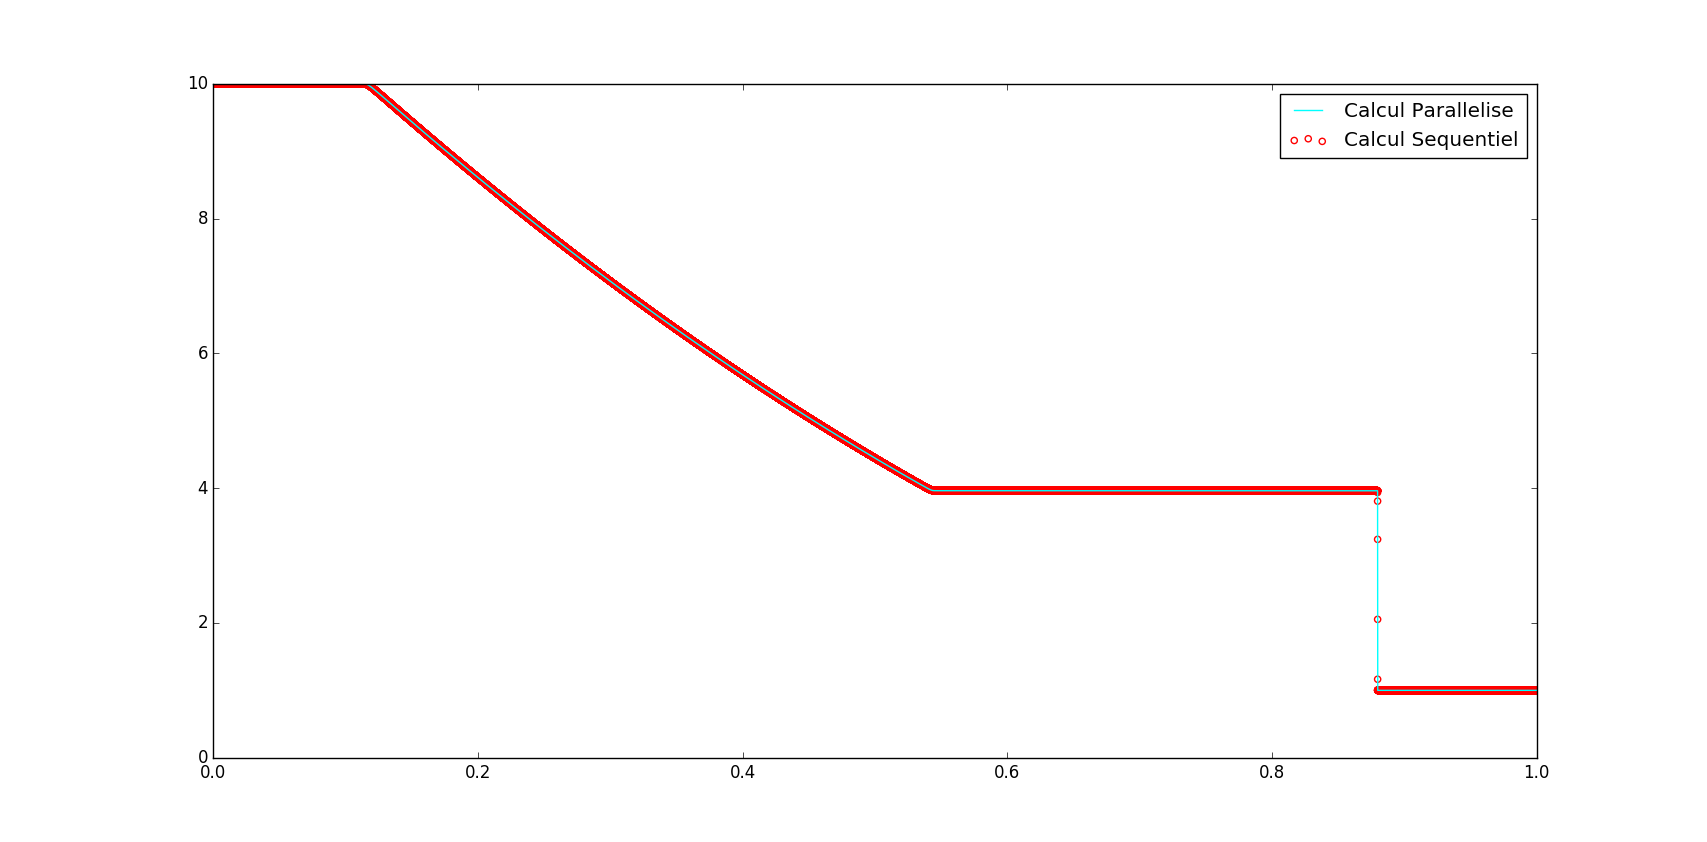
\includegraphics[width = 16cm, height = 10.5cm]{/home/saura/Documents/Latex_files/Pic/seq_par.png}
\end{figure}

L'approximation est bonne, elle est même optimale la droite cyan semble passer par le centre des cercles symbolisant que la courbe du calcul séquentiel se superpose à celle du calcul parallélisé. Nous sommes donc sûrs que la parallélisation n'a pas perdu d'informations et que nous avons bien procédé du point de vue calcul. Maintenant nous allons discuter de notre travail du point de vue efficacité de parallélisation. Voici un tableau recensant les temps mesurés en fonction du nombre de CPU.

 \begin{table}[ht!]  
 \centering
 \begin{tabular}{|l|c|r|}
 
  \hline
  Nombre de CPU & Temps de calcul (en s) & Efficacite : T(1)/T(i)\\
  \hline
  1 (seq) & 1190 & 1\\
  2 & 516 & 2.34\\
  3 & 340 & 3.51\\
  4 & 253 & 4.70\\
  5 & 216 & 5.51\\
  6 & 182 & 6.54\\
  7 & 149 & 7.99\\
  8 & 130 & 9.15\\
  \hline
\end{tabular}
\caption{Tableaux de valeurs permettant de discuter sur l'efficacité de la parallélisation}
\label{tabtab}
\end{table}

Les valeurs de ce tableau sont surprenantes car elles laisseraient supposer une "\textit{sur-parallélisation}". Je ne sais pas plus sur ce phénomène mais à mon avis l'évaluation du temps de calcul n'était pas bonne par rapport aux processeurs du cluster sur lequel nous avons lancé les calculs en parallèle. Néanmoins comme on le voit dans la figure suivante, la tendance générale de la courbe semble être une droite. 

\begin{figure}[ht!]
\centering
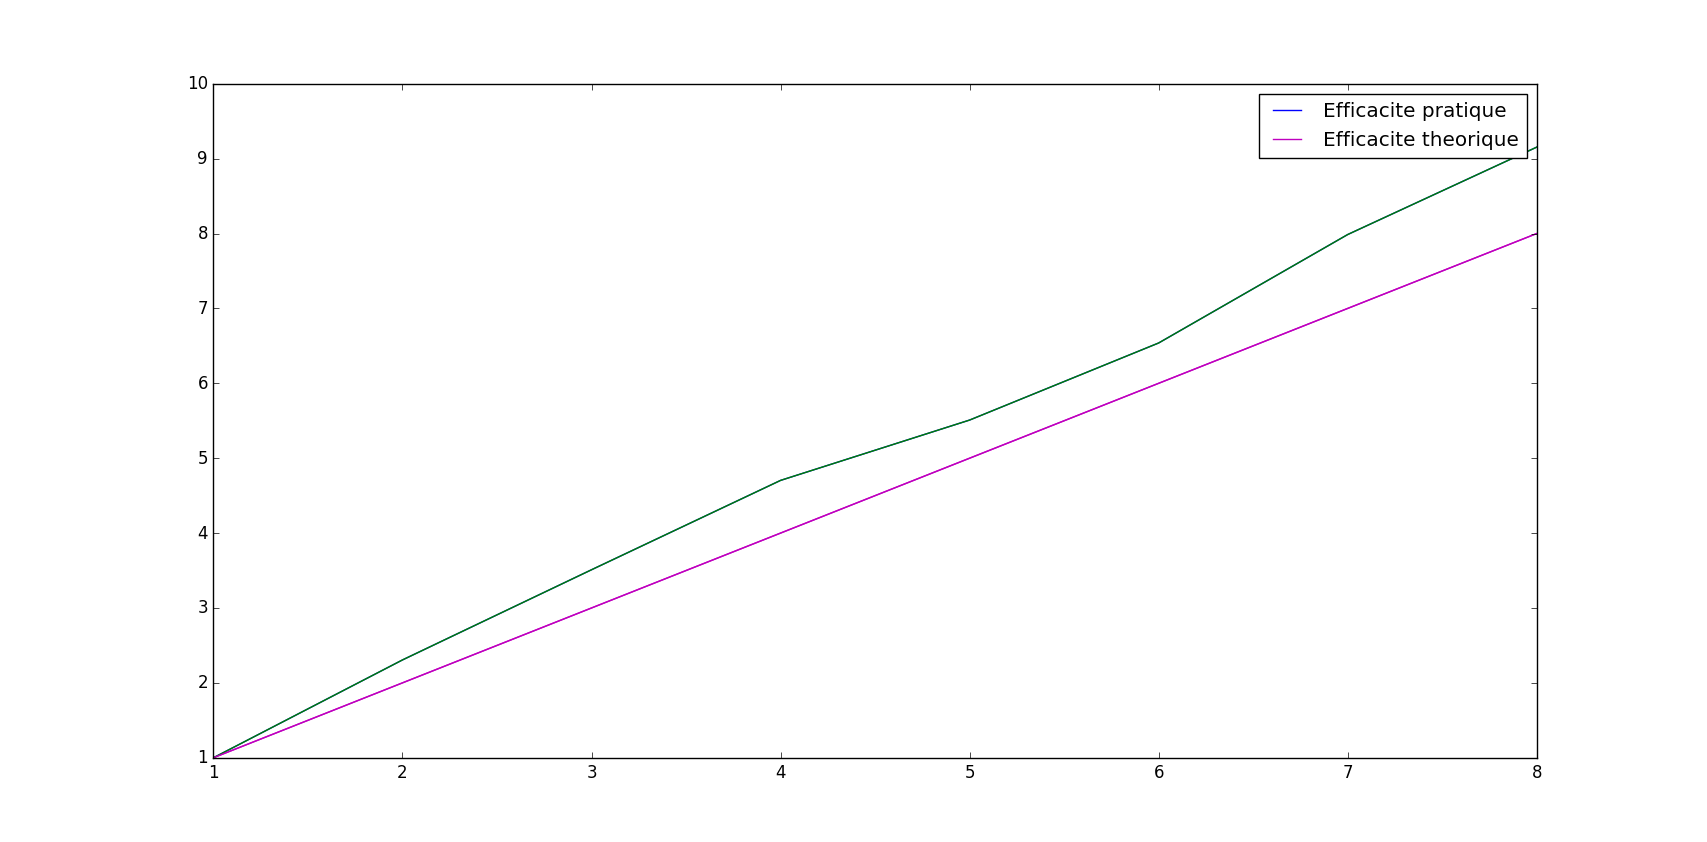
\includegraphics[width = 16cm, height = 10.5cm]{/home/saura/Documents/Latex_files/Pic/eff.png}
\end{figure}

\noindent On vérifie : si on suppose que la première valeur de notre tableau est le double de $516$ soit $1032$, on réécrit notre tableau : 

 \begin{table}[ht!]  
 \centering
 \begin{tabular}{|l|c|r|}
 
  \hline
  Nombre de CPU & Temps de calcul (en s partant de 1032)\\
  \hline
  1 (seq) & 1032\\
  2 & 516 \\
  3 & 344 \\
  4 & 258 \\
  5 & 206.4 \\
  6 & 172 \\
  7 & 147 \\
  8 & 129 \\
  \hline
\end{tabular}
\caption{Tableaux de valeurs si on fixe le premier temps comme le double de 516.}
\label{tabtab2}
\end{table}
On trace alors les différences entre les deuxièmes colonne des tableaux pour voir si les temps de parallélisation se rapproche des valeurs "ajustées" calculées dans le tableau (\ref{tabtab2}) (figure page suivante)

\pagebreak

\begin{figure}[ht!]
\centering
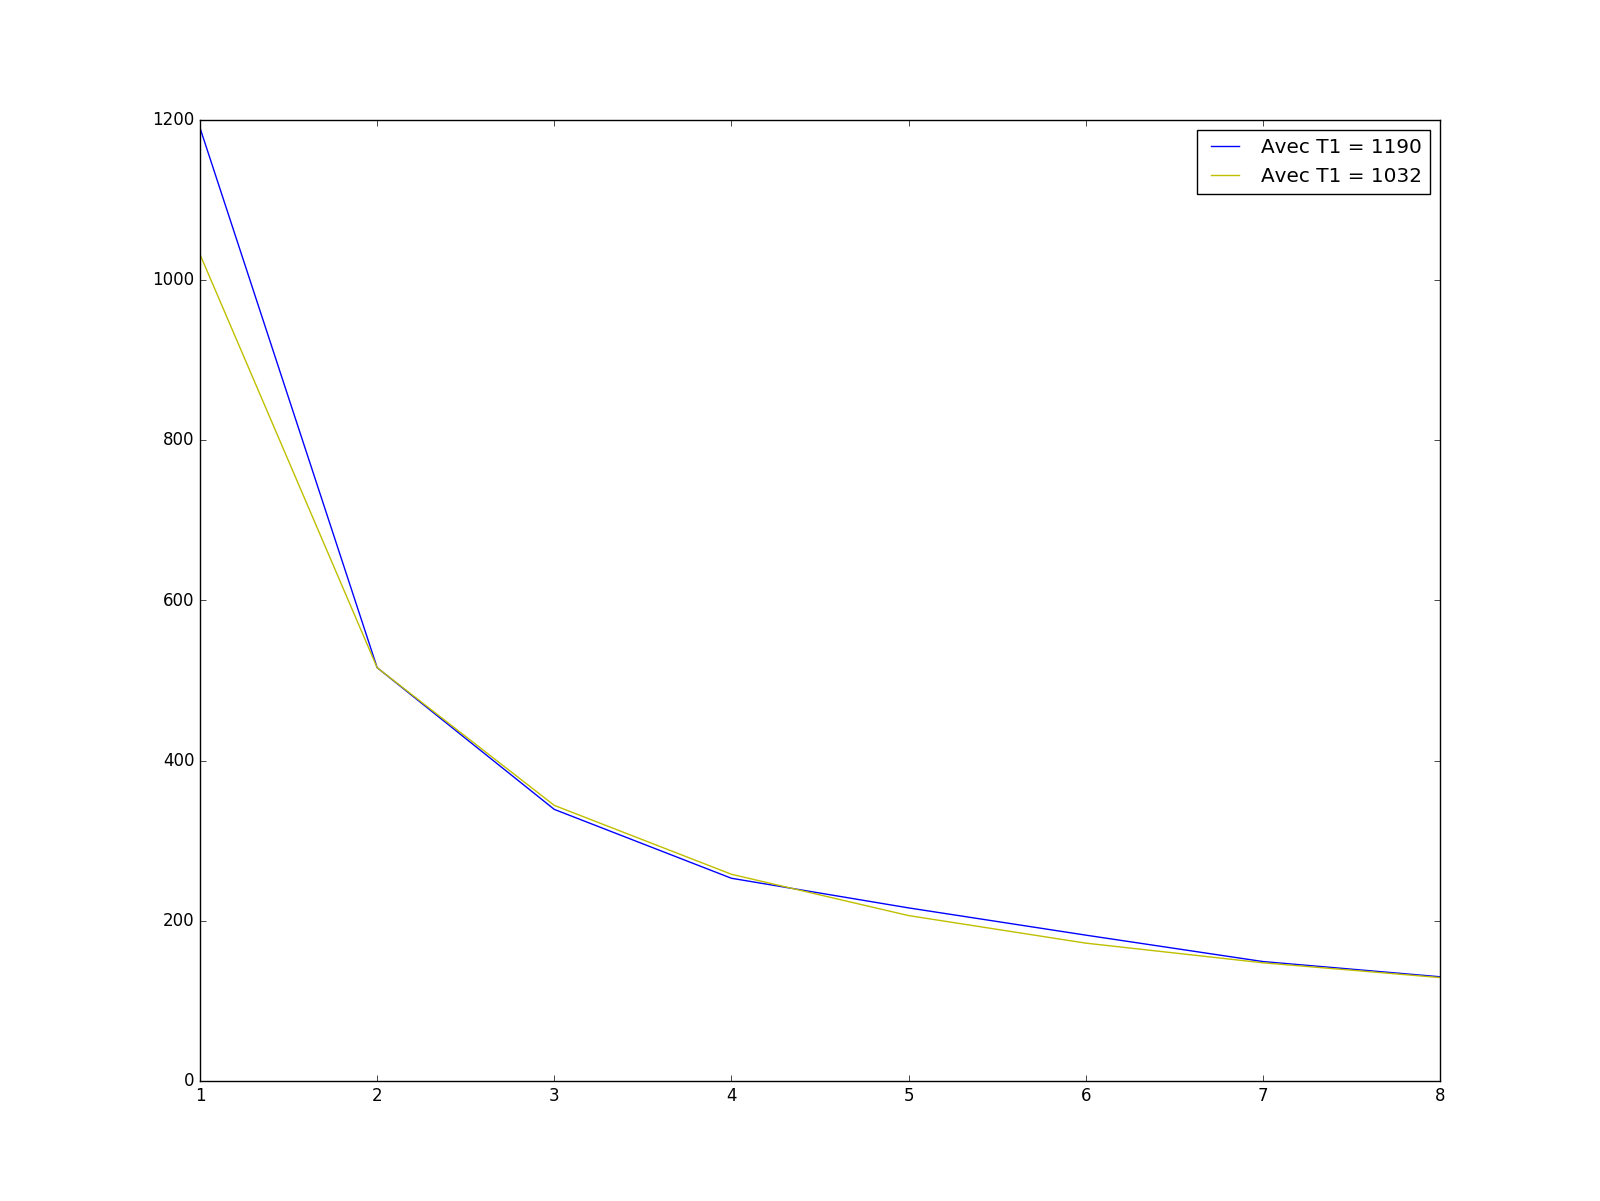
\includegraphics[width = 16cm, height = 10.5cm]{/home/saura/Documents/Latex_files/Pic/comp_t_th.png}
\end{figure}
Les valeurs sont assez proches ce qui nous laissent imaginer que notre parallélisation est assez efficace sans être parfaite non plus.\\

\navy \section*{Conclusion du rapport} \bk
Dans ce rapport nous avons essayé d'être le plus clair possible concernant notre stratégie de parallélisation. Nous avons consciemment "ellipsé" quelque passage de code et nous invitons le lecteur à consulter le code et notamment les commentaires qui sont à mon sens riches en détails car écrits au moment de la construction et de la résolution de certains bugs. Néanmoins subsiste une incertitude : le temps qu'utiliserait un processeur du cluster pour exécuter le programme en séquentiel avec les même paramètres que ceux utilisés pour le calcul parallèle.\\
La parallélisation est \textsc{\textbf{la}} réponse au défi de la physique moderne entre autres disciplines nécessitant des simulations numériques. 
La physique moderne se distingue de la physique des $\underline{\overline{\text{XIX}}}^{\text{ème}}$ et siècles antérieurs par le caractère statistique de celle-ci si ce n'est au minimum le niveau de précision voulu. Nous pouvons citer la turbulence ou les problématiques de marches aléatoires ou encore quantiques, chimiques mais aussi des problèmes plus classiques pour lesquels nous voulons obtenir des résultats plus précis. 
\\ La parallélisation permet en fait d'atteindre des niveaux de description de la physique auxquels les fondateurs de ces disciplines ont forcément dû rêver, et ce pour le même coup de temps de calcul que les codes existants aujourd'hui. Si nous passons de 1190 secondes à 130 secondes avec 8 processeurs, on peut imaginer ce gain de temps (encore plus efficace) à de beaucoup plus grosses échelles. Toutefois, il arrive un moment où la courbe de gain de temps se réduit car il subsistera toujours des parties séquentielles dans un code.\\
 Enfin avec l'avènement du \textit{machine learning}, ou bien des algorithmes comme le \textit{page ranking} des moteurs de recherche, la parallélisation annonce une ère nouvelle, reste à voir si ces technologies serviront les mêmes causes que la dernière révolution énergétique des années 40.

\end{document}